\documentclass[../dissertation.tex]{subfiles}
\begin{document}

\chapter{Systematic Review of Existing Software}
\label{sec:systematic-review}

\section{Aim} 

The goal of the review was to look into several different types of network visualisation software, gathered in Chapter \ref{sec:research}, and as a result, find out more about how it works. The software would be analysed for several characteristics, both related to the visualising of networks and the visualisation of specifically massive networks.

\section{Methodology}
\label{sec:sys-rev-method}

Upon finishing background research and defining a clear aim for the review, a list of criteria and a process had to be created. These would include what would be searched for and tested for in each software package, and instructions on how to go about that testing. The initial task was to split the criteria into several categories and weigh each category as to its importance. 

The first criteria to assess would be how easy it is to get a basic network (5 or 10 nodes) displayed from scratch, from downloading the software and installing it, to understanding it's documentation and finally to getting a network displayed.

Additionally, another criteria was how easy it is to load a network from a file or save a network to a file. These were important as a system would have limited use if it did not allow a user to upload networks, and allowing users to save networks (potentially after it was modified by the system or the user) would mean the network could be loaded in from another system or at a later date. 

The next feature to be analysed was based on interactivity - how easily can a user edit the network to get more useful information out of it. This would include the ability to zoom into a part of the network or being able to pan. A more complex feature (that would be rarely used but would occasionally add valuable information to the user) would be the ability to make it dynamic - showing the change in a network over time (or another parameter). 

A major criteria would then be how well the software would scale up to massive networks - this would include running tests on increasingly large networks and seeing how long the software took, and also if it includes node or edge bundling, or other ways of increasing clarity of massive networks. Time taken to render is also an important statistic, but less critical than the clarity of the massive amounts being displayed. This is perhaps the most vital category as no matter the above features, if the network is not clear for huge numbers of nodes or edges then it does not provide a solution to the problem at hand. An additional feature to increase user clarity would be the ability to view the network in many different layouts (such as Force Directed \cite{fruchterman1991graph} - which is most common layout algorithm - or lesser used algorithms such as spectral layout \cite{beckman1994theory} or arc diagrams \cite{didimo2013graph}), which would give users more flexibility and would often lead to a better understanding of the network. 

This set of criteria, both qualitative and quantitative (to maximise information gathered), was compiled into a list to act as the process for the experiment. This enabled a systematic analysis of the software to take place.

\begin{enumerate}
	\item \textbf{Standalone or library?}\\
	If a software package is standalone then can it be executed (often after it has been installed) without any programming on the user's behalf? If the software comes as a library package then that library will provide an API so one can call functions from the library in their own programs. 
	\item \textbf{Documentation}:
	\begin{enumerate}
		\item Is it easy to understand: is it explained clearly and concisely?
		\item Is it comprehensive: are all aspects of the software fully documented?
		\item Length of time spent reading until confident in using the system: how long was spent reading documentation before programming using the system could begin?
	\end{enumerate}
	\item \textbf{Time until a simple network could be displayed?}\\
	After finishing reading the documentation and starting to use the software, how long did it take to create a hard-coded network with three nodes and two edges? These values were chosen as they represent a very basic network that should be instantaneous to load in nearly all systems, but an understanding of the software is still required to display the network.
	\item \textbf{Can a file be loaded into the system?}\\
	Is there a way to load a file (whether in a standard file format such as JSON or XML, or in a custom file format) into the software? If this is possible, even only in one file format, then a script could be written in order to convert from that file format to whatever necessary file format was needed. 
	\item \textbf{Can a network be exported to a file?}\\
	Is there a way to export a network to a file, in the form of a representation of the network, such as JSON or XML? This would mean that the network could be easily passed between software applications and across a network.
	\item \textbf{Can a network be exported to an image?}\\
	Could the network be exported to a file as an image, such as a PNG or a JPEG? This is useful as images will generally be far smaller than representations of the image in code, such as JSON or XML, and hence are far easier and quicker to send or store on a machine.
	\item \textbf{How long it took to render a network of:}
	\begin{enumerate}
	    \item 30 nodes
	    \item 200 nodes
	    \item 1000 nodes
	    \item 3000 nodes
	\end{enumerate}
	These numbers were chosen as it was expected that all software could handle all of the values, with all software having no trouble with thirty nodes, but software that performs less well being expected to struggle as the number of nodes got into the range of the thousands. 
	\item \textbf{If the software allowed for:}
	\begin{enumerate}
		\item Zooming: if certain parts of a network could be focused on and viewed in more detail.
		\item Panning: the network could be traversed in the x or y axis.
	\end{enumerate}
	\item \textbf{Can a network be dynamic?}\\
	This would allow for information to be viewed across multiple points in time? This allows certain types of information to be visualised far more easily, in particular when data has been been collected over a long time period over which relationships between the data evolve.
	\item \textbf{Does the software included features for displaying huge networks:}
	\begin{enumerate} 
		\item Node Bundling: See section \ref{sec:node_bundling}.
		\item Edge Bundling: See section \ref{sec:edge_bundling}.
		\item Alternative layout options: This includes the ability to change what algorithms decide how the network is laid out.
	\end{enumerate}
	\item \textbf{Can a network be multivariate?}\\
	Does the software support nodes being grouped in some way? This could be in many ways, such as based on shape or colour, and would allow users to distinguish different catagories of data.
	\item \textbf{Is there a possibility of changing graphical settings for the network?}\\
	Can nodes or edges be coloured differently at the users request? This could be done by changing their shape, size, colour or outline?
	\item \textbf{Can a network be displayed in 3D?}\\
	Is there a way to view the network in three dimensions, for example as a globe? This allows for a unique insight into the data and can often make the data a lot easier to comprehend and/or reveal more subtle relationships in the data.
	\item \textbf{Any other idiosyncrasies?}\\
	Is there any other aspect of the software of note that is not identified above?
\end{enumerate}

Each piece of software was evaluated against this criteria, with the goal of both finding out which pieces of software were more successful over many parameters, and also to become more familiar with network visualisation software used in industry.

\section{Data and Results}

After starting to run the experiments, it became clear that two pieces of software from the list above would not be capable of being compared against the criteria stated in Section \ref{sec:sys-rev-method}, which were GUESS and SNAP.

GUESS was software that never left beta, and was last developed in 2007. Having never been released meant that the software had fairly little documentation and what it did have was not comprehensive. On top of this, the wiki created for it was no longer hosted online which meant many of the links to documentation on the website were broken. Despite it looking promising, it became clear it would not be usable.

SNAP could not be compared to much of the criteria as the purpose of it is to analyse and manipulate networks, as opposed to visualising them. However, time was spent reading it’s documentation and going through all the sample code snippets to understanding how the software worked to some degree. The reason this was done was that it both felt important to have some knowledge of how network manipulation software worked, and also depending on the direction the project took, network manipulation may well be used in order to bundle edges or nodes in order to increase performance of massive networks.

The rest of the software however was analysed against the above criteria and the results are documented below.

\subsection{Gephi}

This was the first software package that was as expected, and was fairly easy to test, use and was well documented. After about half an hour it was understood how the system worked and how to make simple networks. Additionally, networks could be loaded and saved from many formats (CSV, GDF, QML, GraphML, net, etc.), and also export to an image or document (PNG, PDF or SVG). It supported zooming, panning, and displaying information dynamically. It also included customisable layout options, some of which would be beneficial for visualising massive networks, although there was no explicit support for them. Additionally, there was the ability to change graphical settings, have the data visualised in 3D, and have a multivariate network. It is written in Java.

\subsection{Graphviz}

Graphviz, ``collection of graph drawing tools'' \cite{ellson2001graphviz}, was difficult to test as it is a collection of software as opposed to a single package. Most of the packages were not fit for purpose, often displaying data in charts, for example. The package I ended up testing was ``sfdp''. Although it fitted most of the criteria and claimed to support large networks, it turned out to be very focused on visualising far smaller networks with little support for anything of a few thousand nodes or more. The documentation was clear, and the software had the ability to import and export a to very large amount of file formats. It also supported zooming/panning, but the user interface clearly was not build around supporting large networks, with information becoming very unclear quickly - see Figure \ref{fig:graphviz}. There was also no explicit support for visualising massive networks. It is predominantly written in C.

\begin{figure}
    \centering
    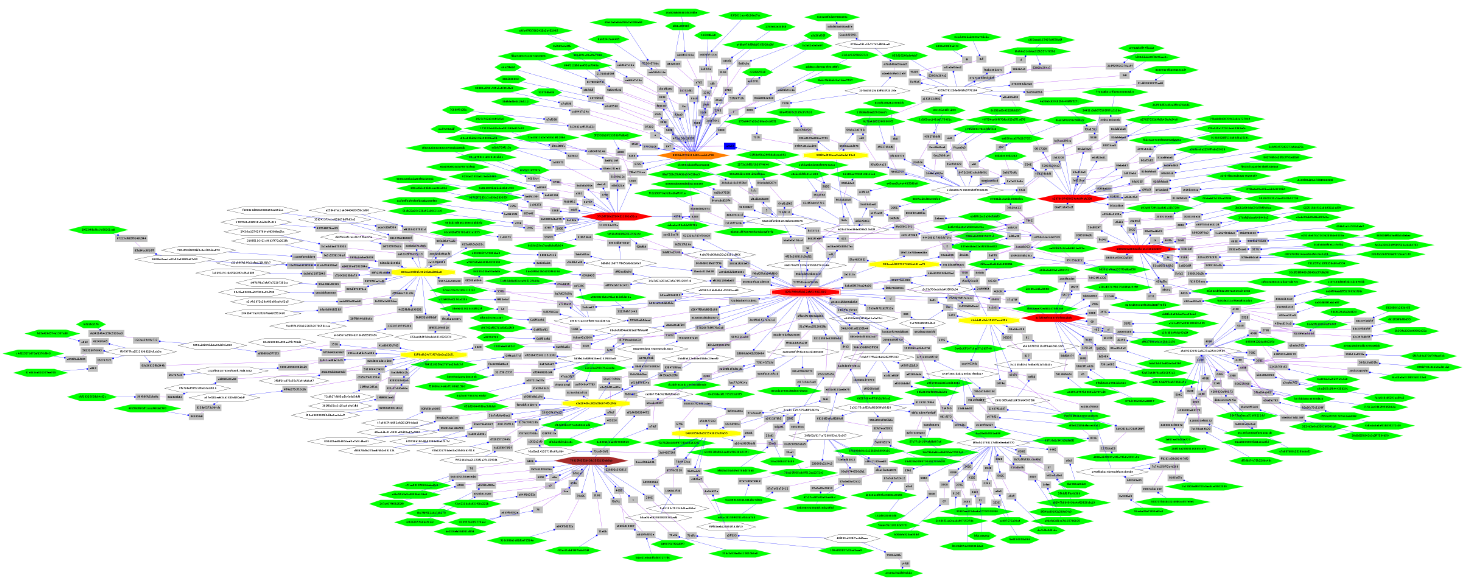
\includegraphics[width=17cm]{4/graphviz}
    \caption{this shows how Graphviz's user interface is focused towards smaller networks of up to a thousand nodes or so, with a lot of detail being shown that becomes impossible to see quickly.}
    \label{fig:graphviz}
\end{figure}

\subsection{Tulip}

Tulip is an information visualisation framework that lets users both visualise and analyse the data. It was very easy to use and thoroughly documented, and allowed for easy importing and exporting of networks. Additionally, it performed very well, allowing for 3000 nodes to be visualised nearly instantly. It also included edge bundling and 'clustering' (a type of node bundling) to improve visualisations of massive amounts of data. It is written in C++ and has a full Python wrapper.

\subsection{D3.js}

D3.js is a JavaScript library for data visualisation. The library is far more flexible than the rest of the software tested, but requires far more setup to be done by the user. The documentation is good although as a result of D3.js's complexity, the documentation is more complicated than all of the other programs. Importing and exporting data is simple using JSON, and other file formats with slightly greater difficulty. It supports zooming and panning. Also, there are many ways to make it effective at showing massive networks, but this would require research into many different packages and potentially writing a lot of code.

\subsection{Vis.js}

Vis.js is, like D3.js, a JavaScript library for data visualisation. However, unlike D3.js, it is not hugely flexible but much easier to get a basic network setup. The documentation is very good and importing and exporting is easily possible via JSON. It also includes some node bundling options. It does not perform as well as D3.js, with significantly lower rendering times as can be seen in Table \ref{table:render-times}.

\section{Software Comparison}

For the majority of the criteria, all of the software packages performed similarly. All five of the fully analysed network visualisation software provided the functionality of zooming and panning, along with all of the standalone packages (Gephi, GraphViz and Tulip) allowing for users to export to/import from a file, and the two libraries (D3.js and Vis.js) had functions which made it easy to export a network to a file or import from a file. On top of exporting to a standard file format for a network, all of the software allowed for exporting to an image.

See Table \ref{table:render-times} for render the times for each of the different pieces of software.

\begin{table}[H]
    \centering
    \begin{tabular}{|l|l|l|l|l|}
        \hline
                 & \textbf{30 nodes} & \textbf{200 nodes} & \textbf{1000 nodes} & \textbf{3000 nodes} \\ \hline
        Gephi    & \textless 0.1   & \textless 0.1    & 0.2                 & 0.6        \\ \hline
        Graphviz & \textless 0.1   & 0.3                & 1.1                 & 4.5        \\ \hline
        Tulip    & \textless 0.1   & \textless 0.1    & \textless 0.1     & 0.1        \\ \hline
        D3.js    & \textless 0.1   & 0.2                & 1.1                 & 5.3        \\ \hline
        Vis.js   & \textless 0.1   & 1.8                & 4.4                 & 13.6       \\ \hline
    \end{tabular}
    \caption{This shows how long (in seconds) it took each of the different pieces of software to render the specified number of nodes.}
    \label{table:render-times}
\end{table}

See Table \ref{table:documentation} for details on the quality of documentation.

\begin{table}[H]
    \centering
    \begin{tabular}{|l|l|l|l|}
        \hline
                 & \textbf{Easy to Understand} & \textbf{Comprehensive} & \textbf{Time spent until confident} \\ \hline
        Gephi    & \tmark             & \tmark        & 30 minutes                 \\ \hline
        GraphViz & \cmark             & \cmark        & 1 hour                     \\ \hline
        Tulip    & \tmark             & \tmark        & 15 minutes                 \\ \hline
        D3.js    & \cmark             & \tmark        & 1 hour, 30 minutes         \\ \hline
        Vis.js   & \tmark             & \tmark        & 5 minutes                  \\ \hline
    \end{tabular}
    \caption{This shows the quality of the documentation for the different pieces of software.}
    \label{table:documentation}
\end{table}

See Table \ref{table:massive-network} for details what features the software had that support visualising massive networks.

\begin{table}[H]
    \centering
    \begin{tabular}{|l|l|l|l|}
        \hline
                 & \textbf{Massive Network Layout Options} & \textbf{Node bundling} & \textbf{Edge bundling} \\ \hline
        Gephi    & \tmark                         & \cmark        & \cmark        \\ \hline
        GraphViz & \cmark                         & \cmark        & \cmark        \\ \hline
        Tulip    & \tmark                         & \tmark        & \tmark        \\ \hline
        D3.js    & n/a                            & n/a           & n/a           \\ \hline
        Vis.js   & \cmark                         & \tmark        & \cmark        \\ \hline
    \end{tabular}
    \caption{This shows what support each of the software packages had for massive networks. D3.js has n/a in all cells as it does not support these features natively. However, D3 is built on using third party packages and libraries, and some of these support several different massive network solutions.}
    \label{table:massive-network}
\end{table}

Table \ref{table:other_info} presents the data on how long it took to create a simple hardcoded network, whether the network visualisation software supported dynamic networks, if the software included graphical options, if networks were viewable in 3D and if a network could be multivariate.

\begin{table}[ht]
    \centering
    \begin{tabular}{|l|l|l|l|l|l|}
        \hline
                                                                    & \textbf{Gephi} & \textbf{GraphViz} & \textbf{Tulip} & \textbf{D3.js} & \textbf{Vis.js}    \\ \hline
        Time until hardcoded network could be created (minutes)     & 5         & 30         & 1        & 30         & 5         \\ \hline
        Visualisation could be dynamic                              & \tmark    & \cmark     & \tmark   & n/a        & \cmark    \\ \hline
        Graphical Options                                           & \tmark    & \tmark     & \tmark   & \tmark     & \cmark    \\ \hline
        Ability to view in 3D                                       & \tmark    & \cmark     & \tmark   & \tmark     & \tmark    \\ \hline
        Network could be multivariate                               & \tmark    & \tmark     & \tmark   & \tmark     & \cmark    \\ \hline
    \end{tabular}
    \caption{This shows additional information about the network visualisation software. For whether the visualisation could be dynamic, D3 - again - does not support this natively, but with additional libraries, it could.}
    \label{table:other_info}
\end{table}

\section{Conclusion}

Following the process outlined in Section \ref{sec:sys-rev-method} was difficult as a collection of APIs was expected, which could have been easily compared by their distinguishing factors, but most of the software were standalone packages and were more difficult to compare. This highlighted the difficultly in conducting a systematic evaluation as, due to the complexities in comparing such diverse software, the criteria changed several times throughout the evaluation and continually evolved, meaning all previously tested software had to be analysed again. Additionally, only the JavaScript libraries would be directly suitable for SAS as the other pieces of software were standalone applications and could not be be utilised by a web application.

Despite the aforementioned challenges, a lot of useful information was gained throughout the evaluation, from how individual packages work to what techniques software uses to deal with large networks. Given all of the above data and comparisons, Tulip was clearly the best performing software. Like all of the other software, it allows for:
\begin{itemize}
    \item Importing from a file (many file formats supported, including it's own \texttt{.tlp} format)
    \item Exporting to a file (to a similarly large number of supported formats)
    \item Exporting to an image
    \item High quality documentation
    \item Graphical options for the network exist
    \item Networks can be visualised in 3D
    \item Networks can be multivariate
\end{itemize}

However, it also rendered networks significantly faster than the other software, supported displaying massive networks in many ways (such as advanced layout options, node and edge bundling), could visualise dynamic information and the software makes it very easy to generate networks which made testing easier and more informative. 

Additionally, Tulip has a full C++ API, and a full Python wrapper around the C++ API, meaning one can interface with it fully in either of the two languages, and a very simple file format, \texttt{.tlp} (of which more information can be found on their website \cite{tuliptlp}), which means that networks can easily be created by hand or converted to and from its format to other formats such as JSON.

\section{Potential Areas of Development}

As a result of the above research and review, there were several different directions that the project could go. Four ideas that were considered are listed below:

\subsection{Writing Massive Network Algorithms}

One possible choice would be to write several different programs in JavaScript that alter massive networks by any or all of the techniques highlighted in Section \ref{sec:background}. This collection of algorithms would then be analysed for what effect they had on improving visualisations and render times, and would be tested using using D3.js or Vis.js. 

Upon writing these algorithms, they would be tested:
\begin{itemize}
    \item \textbf{In isolation.} What effect that function has on a network in regards to visualisation quality and render times
    \item \textbf{In conjunction with other algorithms.} If combining certain algorithms together leads to a greater improvement
    \item\textbf{ With a large variety of different sizes of networks.} If the algorithm hits a bottleneck after the network contains more than a certain number of nodes, or continues to perform as well as expected.
    \item \textbf{With a variety of sparse or highly interconnected networks.} Some algorithms, for example bundling, may work particularly well with highly interconnected networks, and analysing performance for different levels of connectedness could reveal when it is most often best to use a certain algorithm.
\end{itemize}

For each of the above tests, each run would have it's performance evaluated (from time taken to how much processing power it required and the amount of RAM used) and then what effect it had on the end visualisation (if spending the time to run the algorithm gave any minor or notable benefit to the visualisation of the network).

\subsection{Evaluation of existing systems}

For each of the standalone systems evaluated in Section \ref{sec:systematic-review} - which were Gephi, GraphViz and Tulip - explore where each of the packages begin to struggle to display networks clearly or quickly and why. This would include analysing the amount of time taken to run on different datasets, and for massive datasets, discover what task in particular makes it take as long as it would to display. Possible reasons could be that the network can't fit in RAM so data is constantly being put onto and pulled off of backing storage, or that algorithms have exponential performance which is negligible for a while but as networks get massive this performance starts to take it's toll. 

Additionally, it would look at how effective the visualisations that created were at imparting knowledge to the user. This analysis would both take into account the quality of the visualisation baring in mind how long it took, and also how clear the visualisation was, regardless of time taken to create it. 

\subsection{Exploration of database visualisation systems}

Another option would be to look into different database visualisation systems. Many database software solutions incorporate visualisation into them, and/or support writing your own visualisation programs and linking them to the information in the database. This path could be interesting as most databases can handle a very large amount of data, and hence storing the data would be an issue that does not need to be considered. 

\subsection{Creation of a web application to load and manipulate massive networks}

A web application would be created that enable users to upload and visualise massive networks. This application would allow users to request to visualise a network and give them the choice to apply one or several bundling algorithms to the data. This would result in faster network transfers and significantly reduced rendering times, but these benefits would be at the cost of processing the network on the server.

\section{Project Direction}

It was decided that \textbf{creating a web application to load and manipulate massive networks} is how the project should progress. This would result in users being able to access visualisations of many massive networks without requiring a huge amount of computational power. This could benefit both employees of a business and business clients in many ways. Users who are required to analyse data would be able to use systems with lower specifications which would result in lower costs for companies using the service and more potential customers for companies selling the service. Most importantly, any user of the system would additionally be able to better visualise and understand massive networks.

\end{document}